\newpage
\subsubsection{Creating EReferences with MOSL}
\texHeader
\hypertarget{static:references tex}{}

In MOSL, the declaration of a reference is simple; the syntax is made up of four parts:  {\small{\texttt{[Aggregation Type][Navigation
Name](Multiplicity):[Role]}}}. A simple reference is defined with an arrow operator, while a contained reference is a sideways diamond and arrow combination.

% Edit me
To avoid redundancies in your code, it's important to know that both types automatically update the other role involved in the reference, which means you only
have to declare a direction once.


\begin{itemize}

\item[$\blacktriangleright$] Open \texttt{Box} class in the editor and add a \emph{container reference} named \texttt{containedPartition} with a multiplicity of zero
to infinite, of type \texttt{Partition} (Fig.~\ref{fig:cpartitionReference}). This means {\bf THAT}.

\begin{figure}[htbp]
	\centering
  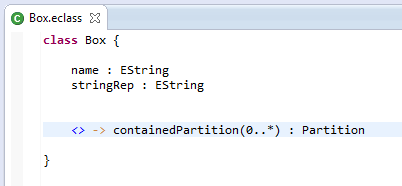
\includegraphics[width=0.6\textwidth]{eclass_box}
	\caption{Creating a \emph{contained reference} in \texttt{Box}}
	\label{fig:cpartitionReference}
\end{figure} 

\item[$\blacktriangleright$] Now add a \emph{simple reference} to \texttt{Partition}. Name it \texttt{box}, and allow it to hold up to one \texttt{Box}
(Fig.~\ref{fig:boxReference}). This means {\bf THAT}.

\begin{figure}[htbp]
	\centering
  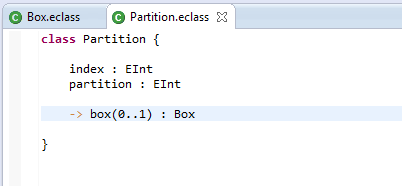
\includegraphics[width=0.6\textwidth]{eclass_partition}
	\caption{Creating a \emph{simple reference} in \texttt{Partition}}
	\label{fig:boxReference}
\end{figure} 

\item[$\blacktriangleright$] Congratulations, you have just built your first pair of EReferences. This pair is also known as a \emph{Bidirectional
EReference}! To see how this is depicted visually, check out Fig.~\ref{fig:ereference_completed} in the previous subsection.

\newpage

\item[$\blacktriangleright$] Now, lets create another EReference pair, or bidirectional EReference, between \texttt{Partition} and \texttt{Card}. If you think
about it, it's really not all that different than the relation between \texttt{Box} and \texttt{Partition}. In fact, it's not different at all! A
\texttt{Partition} should be able to hold an unlimited amount of \texttt{Card}s, but a \texttt{Card} should only be allowed to belong to zero or one
\texttt{Partition}s. Name the two new relations \texttt{containedPartition}, and \texttt{box}.

\item[$\blacktriangleright$] Your classes should now closely resemble Fig.~\ref{fig:almostAllReferences}.

\begin{figure}[htbp]
	\centering
  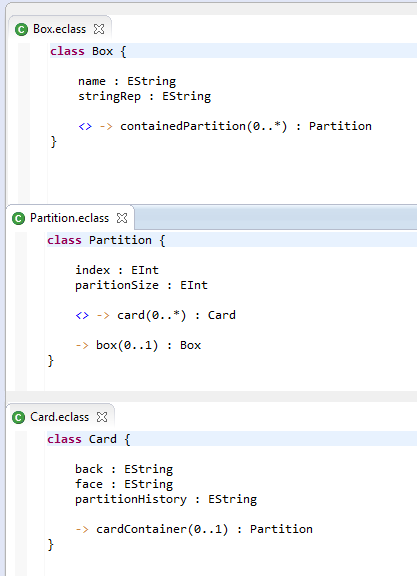
\includegraphics[width=0.65\textwidth]{eclipse_workspaceReferences}
	\caption{The Completed Bidirectional EReferences}
	\label{fig:almostAllReferences}
\end{figure} 

\item[$\blacktriangleright$] The next step is to set up two relations between \texttt{Partition} and itself, so it can shift between the previous and next
partition in the box. Create two new simple references, named \texttt{previous}, and \texttt{next}. Allow them to have a maximum of 1 link each.

\item[$\blacktriangleright$] All of our references are now set up! If you have done everything correctly, your classes should now resemble Fig.~\ref{fig:allReferences}.
To see how all of this is depicted visually, check out Fig.~\ref{fig:ereferences_all} in \hyperlink{sec:static vis}{section 2.1}.

\begin{figure}[htbp]
	\centering
  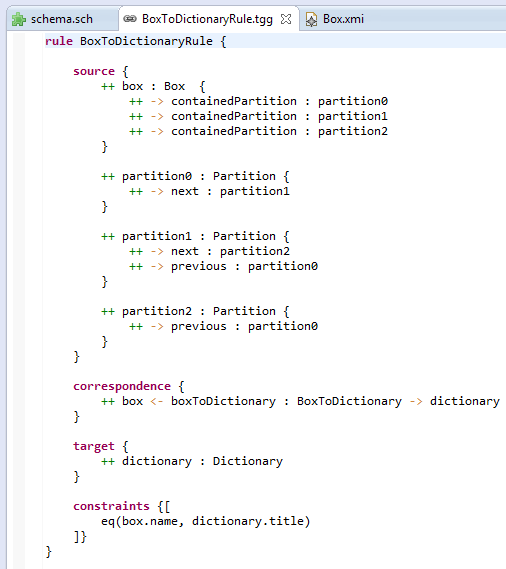
\includegraphics[width=0.6\textwidth]{eclipse_allReferences}
	\caption{All references in Leitner's Learning Box}
	\label{fig:allReferences}
\end{figure} 

\newpage
{\huge Constraints!}
\fancyfoot[R]{$\triangleright$ \hyperlink{static:methods tex}{Next}}
\end{itemize}
